\section{Git Workflow and its relation with the CI/CD Pipeline}

El flujo de trabajo en Git se debe realizar de forma organizada y responsable. La idea bajo una \textit{pipeline} de desarrollo, integración y despliegue continuos (CI/CD) es que, según las acciones que se realicen en unas ramas específicas del repositorio de código, se ejecuten diversas acciones acordes al momento y estado del producto.\\

\vspace{5px}

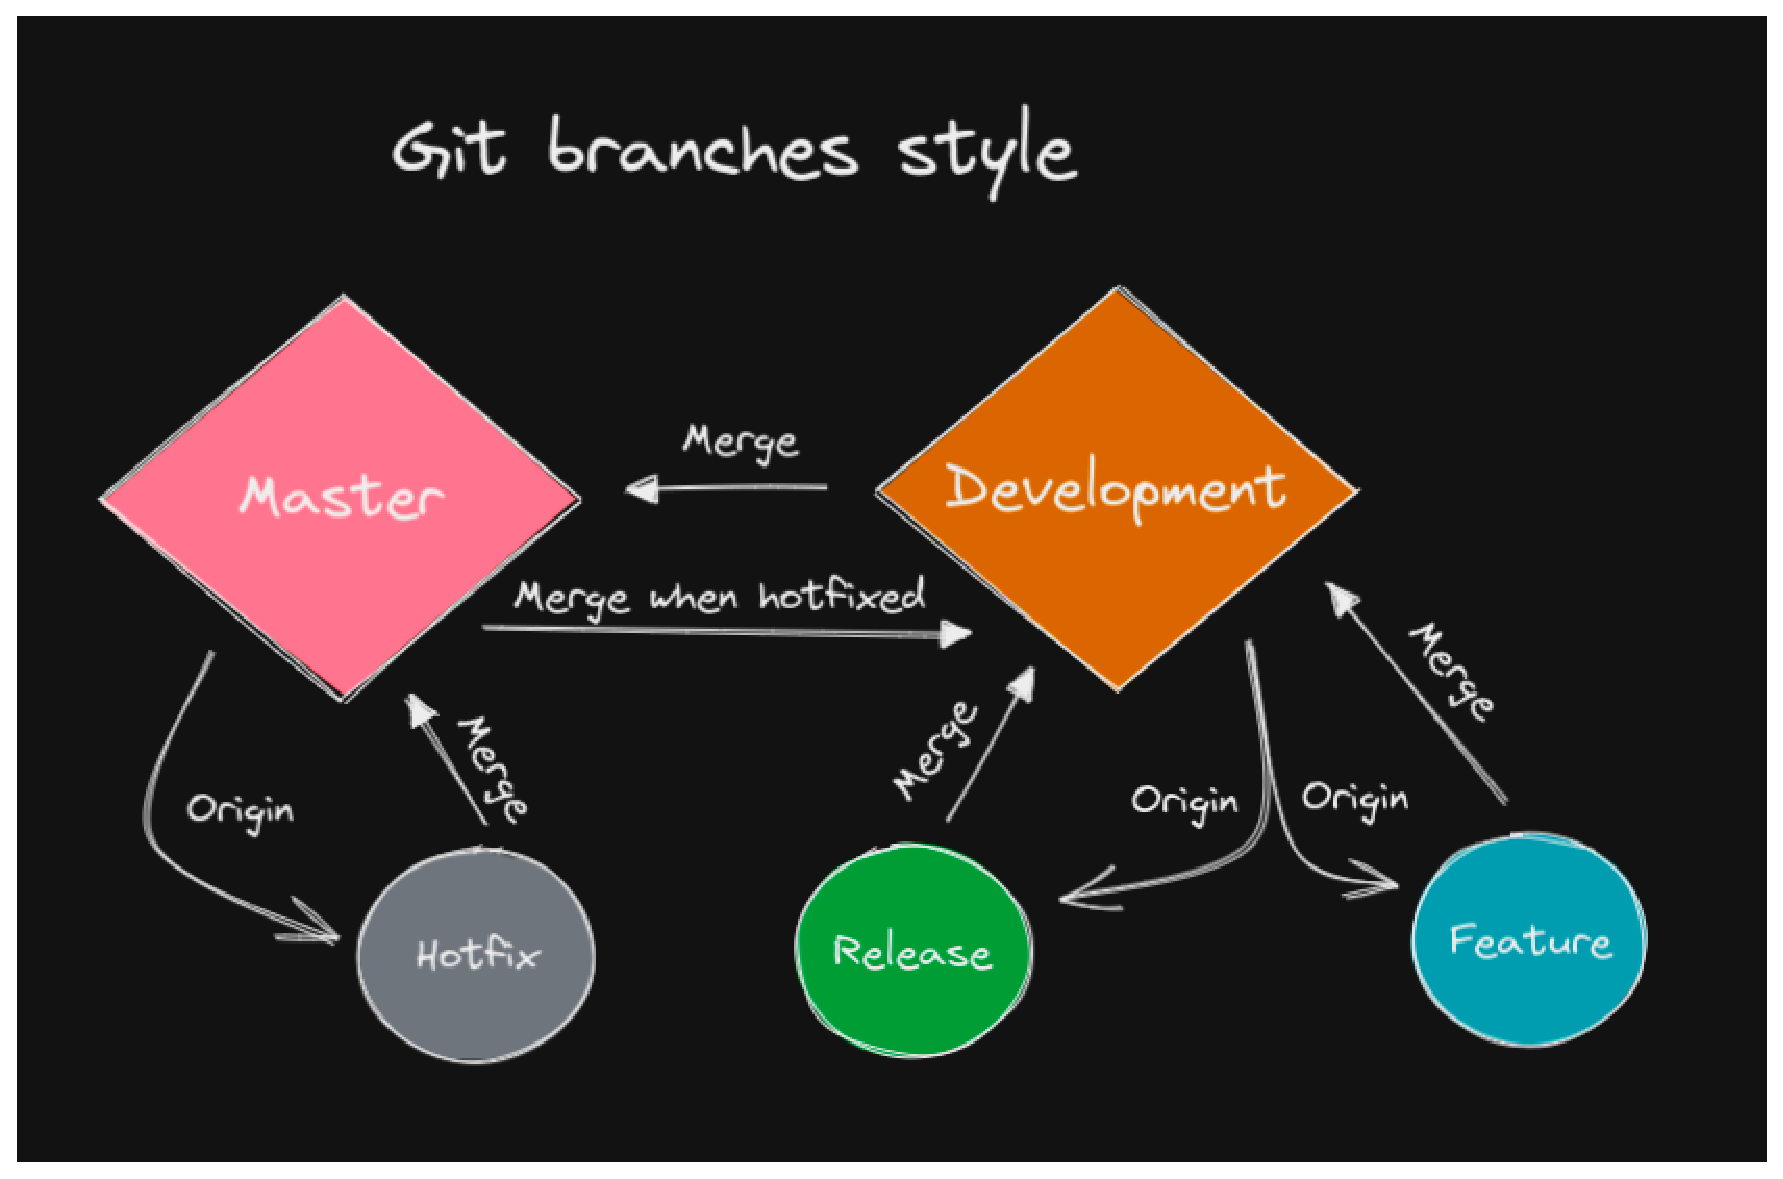
\includegraphics[width=0.9\textwidth]{img/git.eps}

\vspace{10px}

Cada una de las ramas en un repositorio Git se relaciona con una etapa en el ciclo de desarrollo del producto.

\vspace{5px}

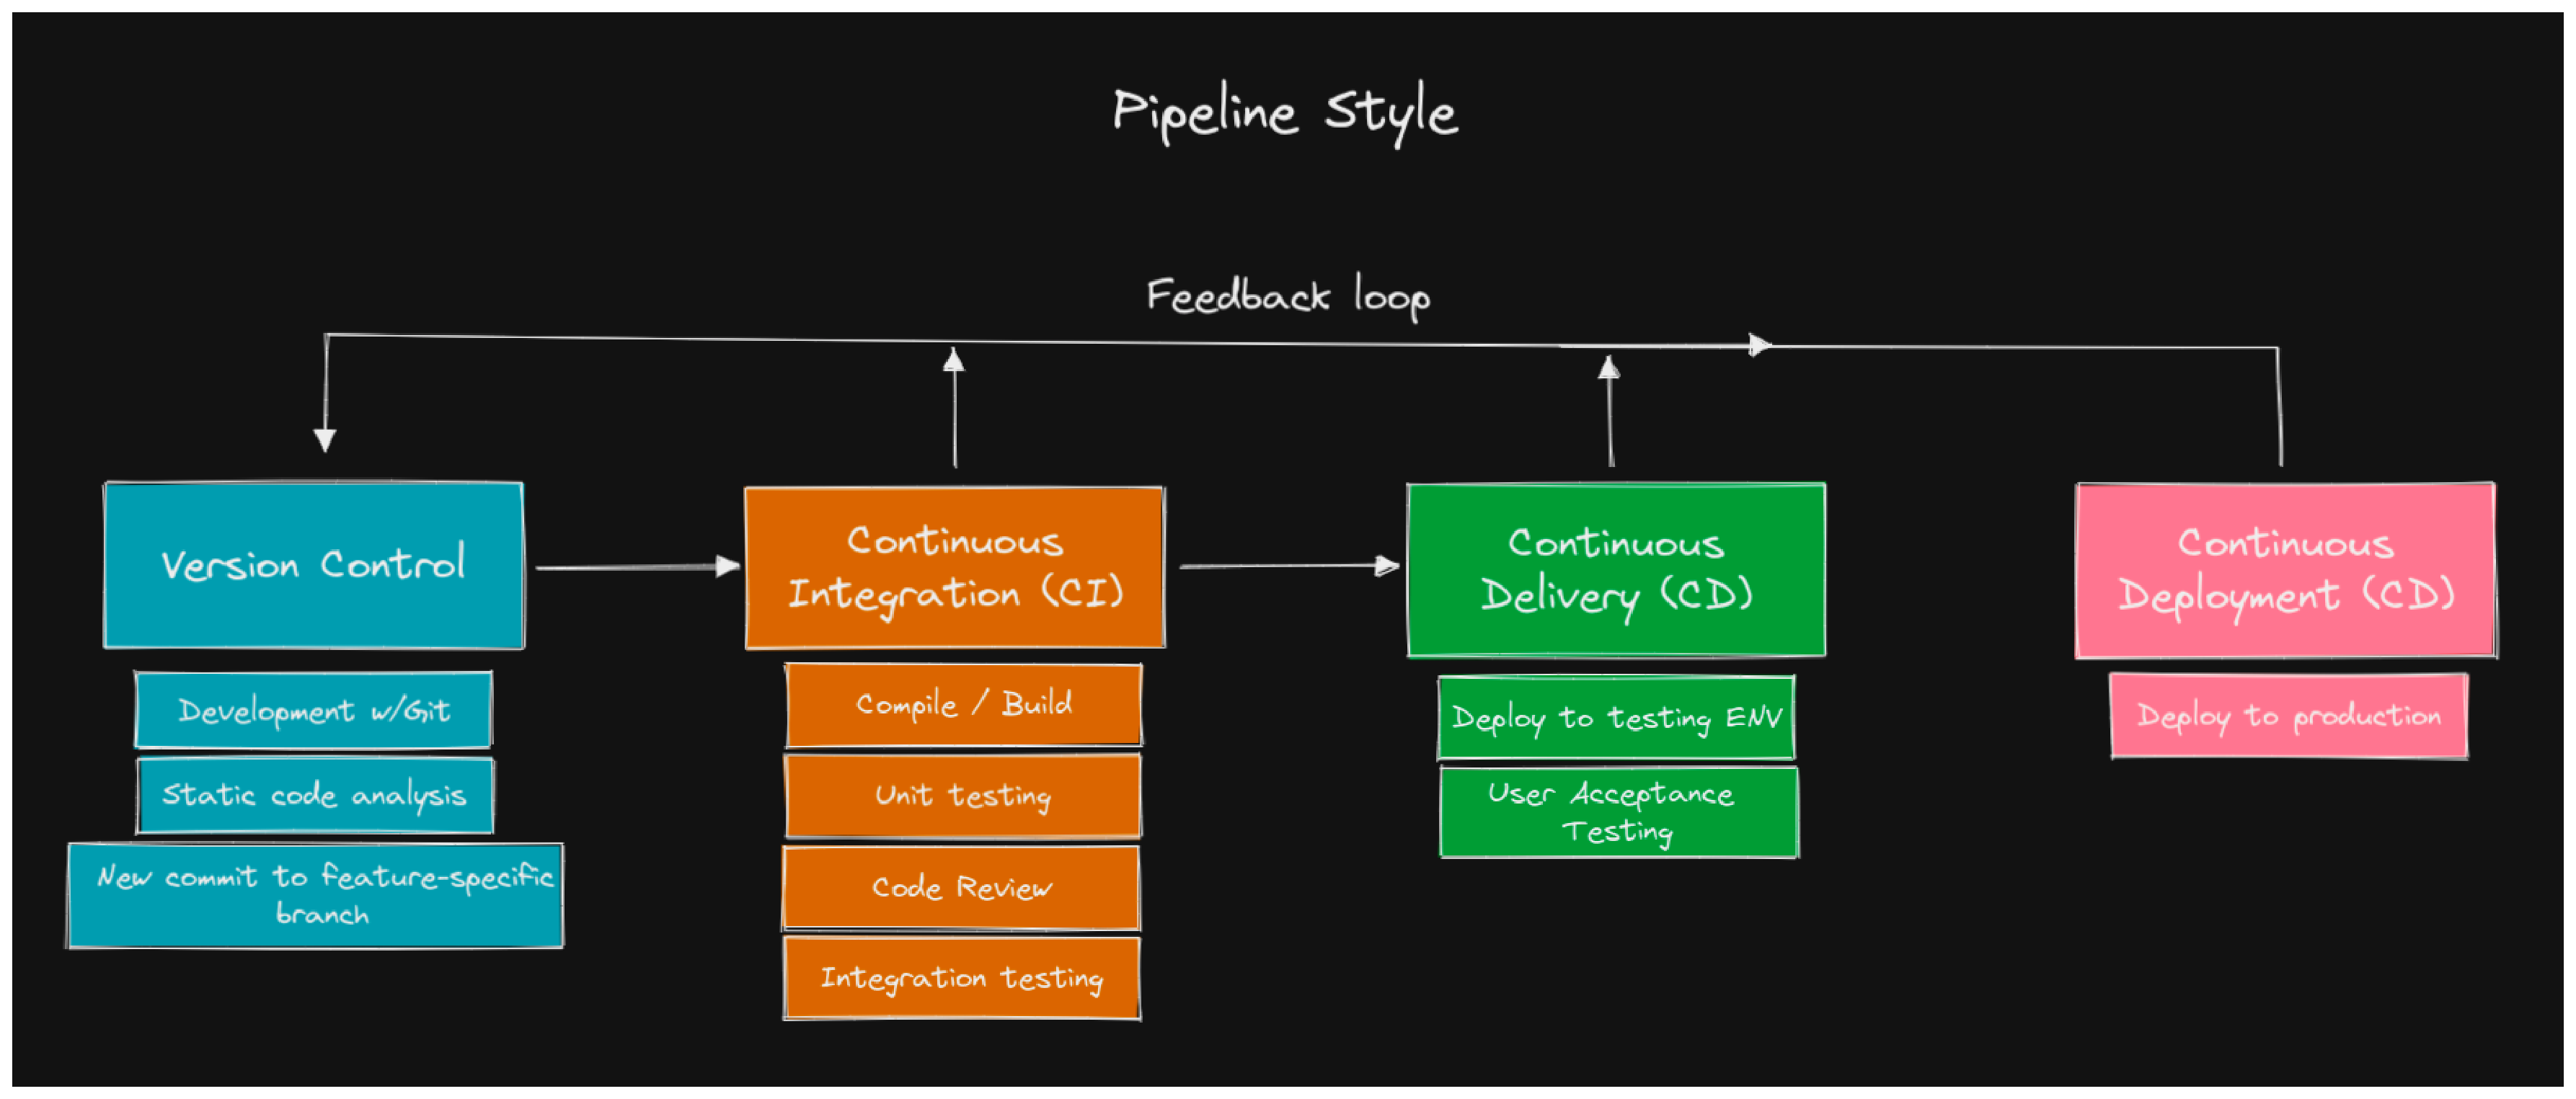
\includegraphics[width=0.9\textwidth]{img/pipeline.eps}

\pagebreak
